\documentclass{book}
\usepackage{blindtext, hyperref, verbatim, minted, graphicx, amssymb, textcomp, enumerate, tcolorbox, newunicodechar, textgreek, wasysym, tipa, eso-pic, lipsum, bbold, dsfont}
\usepackage[margin=1.3in]{geometry}
\usepackage{longtable}
\usepackage{lmodern} % Add this line to use the Latin Modern font
\renewcommand\familydefault{\sfdefault}
\usepackage{fontspec}
\usepackage{newunicodechar}
\usepackage[utf8]{inputenc}
\usepackage{xcolor}

\usepackage{amsthm}

% Theorem styles
\newtheorem{theorem}{Theorem}[section]
\newtheorem{definition}[theorem]{Definition}

\newunicodechar{×}{$\times$}
\newunicodechar{→}{$\rightarrow$}
\newunicodechar{⟨}{$\langle$}
\newunicodechar{⟩}{$\rangle$}
\newunicodechar{↦}{$\mapsto$}
\newunicodechar{∧}{$\wedge$}
\newunicodechar{∨}{$\vee$}
\newunicodechar{∃}{$\exists$}
\newunicodechar{∀}{$\forall$}
\newunicodechar{¬}{$\neg$}

\newunicodechar{ᵃ}{${}^{\texttt{a}}$}
\newunicodechar{ᵇ}{${}^{\texttt{b}}$}
\newunicodechar{ᶜ}{${}^{\texttt{c}}$}
\newunicodechar{ᵈ}{${}^{\texttt{d}}$}
\newunicodechar{ᵉ}{${}^{\texttt{e}}$}
\newunicodechar{ᶠ}{${}^{\texttt{f}}$}
\newunicodechar{ᵍ}{${}^{\texttt{g}}$}
\newunicodechar{ʰ}{${}^{\texttt{h}}$}
\newunicodechar{ⁱ}{${}^{\texttt{i}}$}
\newunicodechar{ʲ}{${}^{\texttt{j}}$}
\newunicodechar{ᵏ}{${}^{\texttt{k}}$}
\newunicodechar{ˡ}{${}^{\texttt{l}}$}
\newunicodechar{ᵐ}{${}^{\texttt{m}}$}
\newunicodechar{ⁿ}{${}^{\texttt{n}}$}
\newunicodechar{ᵒ}{${}^{\texttt{o}}$}
\newunicodechar{ᵖ}{${}^{\texttt{p}}$}
\newunicodechar{ʳ}{${}^{\texttt{r}}$}
\newunicodechar{ˢ}{${}^{\texttt{s}}$}
\newunicodechar{ᵗ}{${}^{\texttt{t}}$}
\newunicodechar{ᵘ}{${}^{\texttt{u}}$}
\newunicodechar{ᵛ}{${}^{\texttt{v}}$}
\newunicodechar{ʷ}{${}^{\texttt{w}}$}
\newunicodechar{ˣ}{${}^{\texttt{x}}$}
\newunicodechar{ʸ}{${}^{\texttt{y}}$}
\newunicodechar{ᶻ}{${}^{\texttt{z}}$}

\newunicodechar{⁰}{${}^{\texttt{0}}$}
\newunicodechar{¹}{${}^{\texttt{1}}$}
\newunicodechar{²}{${}^{\texttt{2}}$}
\newunicodechar{³}{${}^{\texttt{3}}$}
\newunicodechar{⁴}{${}^{\texttt{4}}$}
\newunicodechar{⁵}{${}^{\texttt{5}}$}
\newunicodechar{⁶}{${}^{\texttt{6}}$}
\newunicodechar{⁷}{${}^{\texttt{7}}$}
\newunicodechar{⁸}{${}^{\texttt{8}}$}
\newunicodechar{⁹}{${}^{\texttt{9}}$}

\newunicodechar{⁻}{${}^{\texttt{-}}$}

\newunicodechar{ᵒ}{${}^{\texttt{o}}$}
\newunicodechar{ᵖ}{${}^{\texttt{p}}$}

\newunicodechar{⁻}{${}^{\texttt{-}}$}
\newunicodechar{¹}{${}^{\texttt{1}}$}

\newunicodechar{₀}{${}_{\texttt{0}}$}
\newunicodechar{₁}{${}_{\texttt{1}}$}
\newunicodechar{₂}{${}_{\texttt{2}}$}
\newunicodechar{₃}{${}_{\texttt{3}}$}
\newunicodechar{₄}{${}_{\texttt{4}}$}
\newunicodechar{₅}{${}_{\texttt{5}}$}
\newunicodechar{₆}{${}_{\texttt{6}}$}
\newunicodechar{₇}{${}_{\texttt{7}}$}
\newunicodechar{₈}{${}_{\texttt{8}}$}
\newunicodechar{₉}{${}_{\texttt{9}}$}

\newunicodechar{𝚫}{$\Delta$}

\newunicodechar{𝔸}{$\mathbb{A}$}
\newunicodechar{𝔹}{$\mathbb{B}$}
\newunicodechar{ℂ}{$\mathbb{C}$}
\newunicodechar{𝔻}{$\mathbb{D}$}
\newunicodechar{𝔼}{$\mathbb{E}$}
\newunicodechar{𝔽}{$\mathbb{F}$}
\newunicodechar{𝔾}{$\mathbb{G}$}
\newunicodechar{ℍ}{$\mathbb{H}$}
\newunicodechar{𝕀}{$\mathbb{I}$}
\newunicodechar{𝕁}{$\mathbb{J}$}
\newunicodechar{𝕂}{$\mathbb{K}$}
\newunicodechar{𝕃}{$\mathbb{L}$}
\newunicodechar{𝕄}{$\mathbb{M}$}
\newunicodechar{ℕ}{$\mathbb{N}$}
\newunicodechar{𝕆}{$\mathbb{O}$}
\newunicodechar{ℙ}{$\mathbb{P}$}
\newunicodechar{ℚ}{$\mathbb{Q}$}
\newunicodechar{ℝ}{$\mathbb{R}$}
\newunicodechar{𝕊}{$\mathbb{S}$}
\newunicodechar{𝕋}{$\mathbb{T}$}
\newunicodechar{𝕌}{$\mathbb{U}$}
\newunicodechar{𝕍}{$\mathbb{V}$}
\newunicodechar{𝕎}{$\mathbb{W}$}
\newunicodechar{𝕏}{$\mathbb{X}$}
\newunicodechar{𝕐}{$\mathbb{Y}$}
\newunicodechar{ℤ}{$\mathbb{Z}$}

\newunicodechar{⊣}{\ensuremath{\dashv}}
\newunicodechar{ॱ}{${}^{\cdot}$}
\newunicodechar{𛲔}{${}_{\cdot}$}
\newunicodechar{⇄}{$\rightleftarrows$}
\newunicodechar{⇆}{$\leftrightarrows$}

\newunicodechar{ꜝ}{$\raisebox{1ex}{\scalebox{0.5}{\texttt{!}}}$}
\newunicodechar{ꜞ}{$\raisebox{1ex}{\scalebox{0.5}{\texttt{¡}}}$}

\newunicodechar{𝟙}{$\mathbb{1}$}
\newunicodechar{∘}{$\circ$}

\newunicodechar{𝟏}{${\bold{1}}$}
\newunicodechar{⭢}{$\longrightarrow$}
\newunicodechar{•}{${\bullet}$}
\newunicodechar{∙}{${\bullet}$}

\newunicodechar{⇉}{$\rightrightarrows$}
\newunicodechar{よ}{$
\includegraphics[width=0.27cm,height=0.27cm]{yon.png}$}

\newunicodechar{∼}{$\sim$}
\newunicodechar{≃}{$\simeq$}
\newunicodechar{≅}{$\cong$}
\newunicodechar{∞}{$\infty$}

\newunicodechar{α}{$\alpha$}
\newunicodechar{β}{$\beta$}
\newunicodechar{γ}{$\gamma$}
\newunicodechar{δ}{$\delta$}
\newunicodechar{ε}{$\epsilon$}
\newunicodechar{η}{$\eta$}
\newunicodechar{ζ}{$\zeta$}
\newunicodechar{θ}{$\theta$}
\newunicodechar{ι}{$\iota$}
\newunicodechar{μ}{$\mu$}
\newunicodechar{κ}{$\kappa$}
\newunicodechar{λ}{$\lambda$}
\newunicodechar{ρ}{$\rho$}
\newunicodechar{π}{$\pi$}
\newunicodechar{σ}{$\sigma$}
\newunicodechar{τ}{$\tau$}
\newunicodechar{υ}{$\upsilon$}
\newunicodechar{φ}{$\phi$}
\newunicodechar{ψ}{$\psi$}
\newunicodechar{χ}{$\chi$}
\newunicodechar{ω}{$\omega$}



\makeatletter
\newcommand*{\shifttext}[2]{\settowidth{\@tempdima}{#2}\makebox[\@tempdima]{\hspace*{#1}#2}}
\makeatother
\definecolor{Red}{cmyk}{0.1, 0.70, 0.65, 0.00, 1.00}
\definecolor{Blue}{cmyk}{0.9, 0.2, 0.2, 0.00, 1.00}
\definecolor{Yellow}{cmyk}{0.0, 0.00, 0.7, 0.00, 0.5}
\definecolor{Green}{cmyk}{0.6, 0.0, 0.6, 0.00, 1.00}
\definecolor{Purple}{cmyk}{0.8, 0.3, 0.3, 0.00, 1.00}
\definecolor{Orange}{cmyk}{0.0, 0.3, 0.7, 0.00, 1.00}
\definecolor{Grey}{cmyk}{0.13, 0.13, 0.13, 0.00, 1.00}
\newcounter{definitioncounter}
\setcounter{definitioncounter}{1}
\newcounter{theoremcounter}
\setcounter{theoremcounter}{1}
\newcounter{printcounter}
\setcounter{printcounter}{1}
\newcounter{examplecounter}
\setcounter{examplecounter}{1}
\newcounter{ccounter}
\setcounter{ccounter}{1}
\newcounter{pcounter}
\setcounter{pcounter}{1}
\newcounter{lcounter}
\setcounter{lcounter}{1}
\newcounter{sectioncount}
\newcounter{subsectioncount}
\setcounter{sectioncount}{1}
\renewcommand{\section}[1]{\newpage\ \\ \ \\ \begin{center} \scalebox{1.5}{\texttt{\thesectioncount . #1}} \stepcounter{sectioncount} \setcounter{subsectioncount}{1} \end{center} \begin{center} \ \\ \ \\ \thispagestyle{empty} \end{center}}
\renewcommand{\subsection}[1]{\texttt{\thesubsectioncount . #1} \stepcounter{subsectioncount}}
\renewcommand{\backslash}{\reflectbox{\texttt{/}}}



\renewcommand{\chapter}[1]{
\newpage
{
\Huge 
\begin{center}
\ \\
\ \\
\thispagestyle{empty}
\texttt{#1}
\end{center}}
\ \\
\ \\
}

\begin{document}

\thispagestyle{empty} 

\AddToShipoutPicture*
    {\put(545,720){\href{http://www.linearlibrary.net}{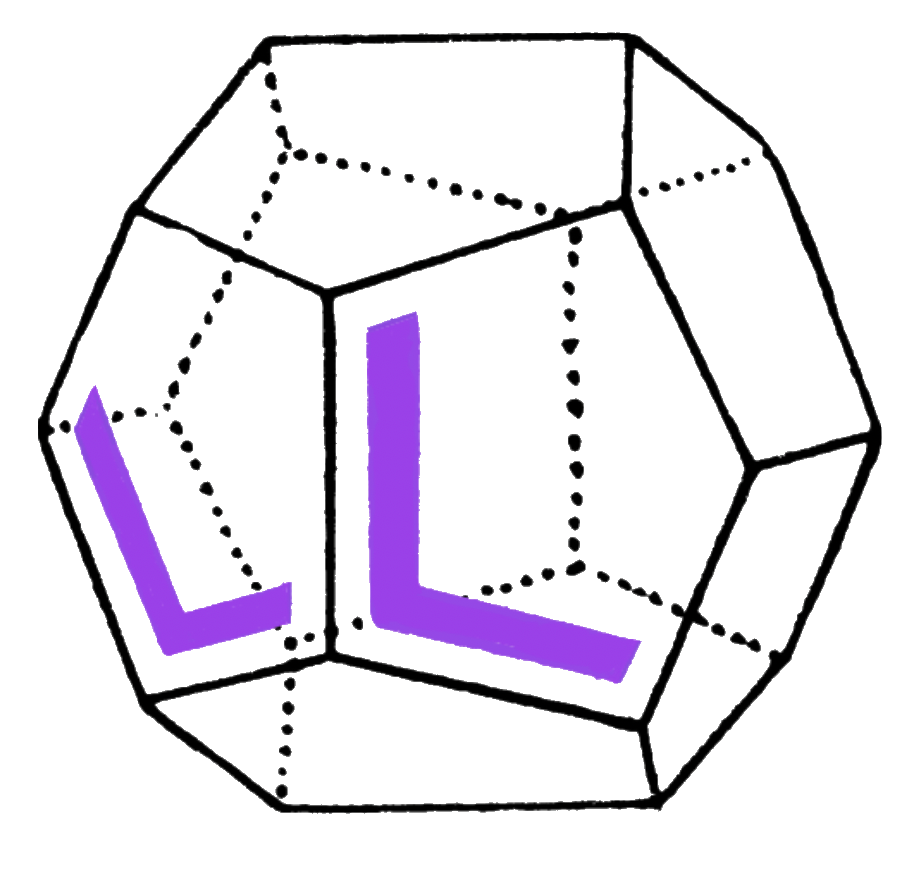
\includegraphics[width=2cm,height=2cm]{ll.png}}}}

\AddToShipoutPicture*
  {\put(465,767){\href{https://github.com/unstableholonomy/TheLaxWhiteheadTheoremforCoglobularLocallyCompactLocales
/blob/main/TheLaxWhiteheadTheoremforCoglobularLocallyCompactLocales
.py}{\raisebox{-0.198 em}{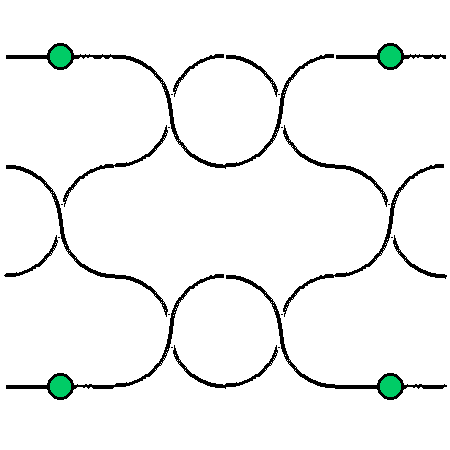
\includegraphics[width=0.35cm,height=0.35cm]{stringdiagrampicture.png}}\texttt{ Braid group}}
  }}

\AddToShipoutPicture*
  {\put(465,752){\href{https://ncatlab.org/nlab/show/enriched+category}{\raisebox{-0.168 em}{
\includegraphics[width=0.33cm,height=0.33cm]{nlablogo.png}}\texttt{ nLab}}\\
  }}

\AddToShipoutPicture*
  {\put(465,737){\href{https://en.wikipedia.org/wiki/Enriched_category}{\texttt{\raisebox{-0.158 em}{
\includegraphics[width=0.38cm,height=0.30cm]{wikipedialogo.png}} Wikipedia}}\\
  }}

  \AddToShipoutPicture*
  {\put(465,722){\href{https://github.com/CQTS}{\texttt{\raisebox{-0.178 em}{
\includegraphics[width=0.32cm,height=0.32cm]{cqtslogo.png}} CQTS}}
  }}


\AddToShipoutPicture*
  {\put(375,767){\href{https://github.com/unstableholonomy/TheLaxWhiteheadTheoremforCoglobularLocallyCompactLocales
/blob/main/TheLaxWhiteheadTheoremforCoglobularLocallyCompactLocales
.lean}{\texttt{\raisebox{-0.1 em}{
\includegraphics[width=0.30cm,height=0.30cm]{leanlogo.png}} Lean file}}}}

\AddToShipoutPicture*
  {\put(375,752){\href{https://github.com/unstableholonomy/TheLaxWhiteheadTheoremforCoglobularLocallyCompactLocales
/blob/main/TheLaxWhiteheadTheoremforCoglobularLocallyCompactLocales
.agda}{\texttt{\raisebox{-0.09 em}{
\includegraphics[width=0.33cm,height=0.31cm]{agdalogo.png}} Agda file}}}}

\AddToShipoutPicture*
  {\put(375,737){\href{https://github.com/unstableholonomy/TheLaxWhiteheadTheoremforCoglobularLocallyCompactLocales
/blob/main/TheLaxWhiteheadTheoremforCoglobularLocallyCompactLocales
.v}{\texttt{\raisebox{-0.17 em}{
\includegraphics[width=0.31cm,height=0.34cm]{coqlogo.png}} Coq file}}}}

  \AddToShipoutPicture*
  {\put(375,722){\href{https://github.com/unstableholonomy/TheLaxWhiteheadTheoremforCoglobularLocallyCompactLocales
/blob/main/TheLaxWhiteheadTheoremforCoglobularLocallyCompactLocales
.thy}{\texttt{\raisebox{-0.2 em}{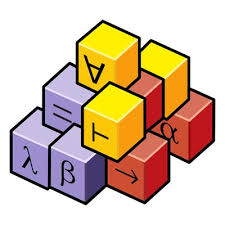
\includegraphics[width=0.34cm,height=0.35cm]{isabellelogo.png}} Isabelle file}}}}


\AddToShipoutPicture*
  {\put(281,767){\href{https://leanprover.zulipchat.com/}{\texttt{\raisebox{-0.1 em}{
\includegraphics[width=0.30cm,height=0.30cm]{leanlogo.png}} Lean Zulip}}}}

\AddToShipoutPicture*
  {\put(281,752){\href{https://agda.zulipchat.com}{\texttt{\raisebox{-0.09 em}{
\includegraphics[width=0.33cm,height=0.31cm]{agdalogo.png}} Agda Zulip}}\\
  }}

\AddToShipoutPicture*
  {\put(281,737){\href{https://coq.zulipchat.com}{\texttt{\raisebox{-0.17 em}{
\includegraphics[width=0.31cm,height=0.34cm]{coqlogo.png}} Coq Zulip}}\\
  }}

  \AddToShipoutPicture*
  {\put(281,722){\href{https://isabelle.zulipchat.com}{\texttt{\raisebox{-0.2 em}{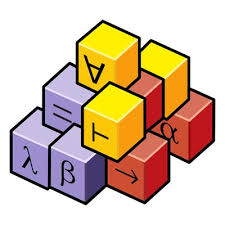
\includegraphics[width=0.34cm,height=0.35cm]{isabellelogo.png}} Isabelle Zulip}}
  }}


\AddToShipoutPicture*
  {\put(185,767){\href{https://linearlibrary.net}{\texttt{linearlibrary.net}}}}

\AddToShipoutPicture*
  {\put(185,752){\href{https://live.lean-lang.org}{\texttt{Leanprover}}}}

\AddToShipoutPicture*
  {\put(185,737){\href{https://github.com/unstableholonomy/TheLaxWhiteheadTheoremforCoglobularLocallyCompactLocales
/blob/main/TheLaxWhiteheadTheoremforCoglobularLocallyCompactLocales
.tex}{\texttt{Latex file}}
  }}

  \AddToShipoutPicture*
  {\put(185,722){\href{https://github.com/unstableholonomy/TheLaxWhiteheadTheoremforCoglobularLocallyCompactLocales
/blob/main/TheLaxWhiteheadTheoremforCoglobularLocallyCompactLocales
.pdf}{\texttt{PDF file}}
  }}



\ \\

\ \\
%LEAN: 
\begin{center}
  \begin{tcolorbox}[width=6in,colback={white},coltitle=white]
  \begin{center}
\scalebox{1.8}{\texttt{The Lax Whitehead Theorem}}\\
\scalebox{1.8}{\texttt{for Coglobular Locally Compact Locales}}\\
\end{center}
\end{tcolorbox}
\end{center}

%LEAN: 
\begin{center}
\begin{tcolorbox}[width=5in,colback={white},colbacktitle=Blue,coltitle=black]

/-

-/

\end{tcolorbox}
\end{center}


%LEAN: 
\begin{center}
\begin{tcolorbox}[width=5in,colback={white},colbacktitle=Blue,coltitle=black]
\begin{minted}[breaklines, escapeinside=||]{lean}

/-
...
-/

\end{minted}
\end{tcolorbox}
\end{center}

\begin{center}
\texttt{Shanghe Chen and Dean Young}
\end{center}
\ \\
\ \\
\thispagestyle{empty}

\newpage

\thispagestyle{empty}

\ \\
\ \\
\ \\
\ \\
\ \\
\ \\
\ \\
\ \\
\ \\
\ \\
\ \\

We wish to acknowledge the collaborative efforts of Shanghe Chen and Dean Young. Together the authors are pursuing these plans as a long term project.\\

\ \\

\newpage
\pagecolor{white}
\color{black}
\ \\
\ \\
\thispagestyle{empty}
\large %%%%%%%% HERE IS THE large LARGE size textsize set text size
\newpage 
\ \\
\ \\
\ \\
\ \\
\ \\
\ \\
\ \\
\ \\
\ \\
\ \\
\ \\
\thispagestyle{empty}



\newpage
\section{Contents}

{
\footnotesize
\begin{longtable}{|| l || l ||} 
\hline
\multicolumn{1}{|c|}{$\texttt{Section}$} & \multicolumn{1}{|c|}{$\texttt{Description}$} \\
\hline
Introduction &  \\
\hline
Contents &  \\
\hline
Unicode &  \\
\hline \hline
... & \\
\hline
ℵʰⁱˡᵇ & Countable strict twocategory of hilbert spaces  \\
\hline \hline
\end{longtable}
}






\newpage
\section{Introduction}


\newpage
\iffalse
░▒▓█▓▒░░▒▓█▓▒░▒▓███████▓▒░░▒▓█▓▒░░▒▓██████▓▒░ ░▒▓██████▓▒░░▒▓███████▓▒░░▒▓████████▓▒░ 
░▒▓█▓▒░░▒▓█▓▒░▒▓█▓▒░░▒▓█▓▒░▒▓█▓▒░▒▓█▓▒░░▒▓█▓▒░▒▓█▓▒░░▒▓█▓▒░▒▓█▓▒░░▒▓█▓▒░▒▓█▓▒░        
░▒▓█▓▒░░▒▓█▓▒░▒▓█▓▒░░▒▓█▓▒░▒▓█▓▒░▒▓█▓▒░      ░▒▓█▓▒░░▒▓█▓▒░▒▓█▓▒░░▒▓█▓▒░▒▓█▓▒░        
░▒▓█▓▒░░▒▓█▓▒░▒▓█▓▒░░▒▓█▓▒░▒▓█▓▒░▒▓█▓▒░      ░▒▓█▓▒░░▒▓█▓▒░▒▓█▓▒░░▒▓█▓▒░▒▓██████▓▒░   
░▒▓█▓▒░░▒▓█▓▒░▒▓█▓▒░░▒▓█▓▒░▒▓█▓▒░▒▓█▓▒░      ░▒▓█▓▒░░▒▓█▓▒░▒▓█▓▒░░▒▓█▓▒░▒▓█▓▒░        
░▒▓█▓▒░░▒▓█▓▒░▒▓█▓▒░░▒▓█▓▒░▒▓█▓▒░▒▓█▓▒░░▒▓█▓▒░▒▓█▓▒░░▒▓█▓▒░▒▓█▓▒░░▒▓█▓▒░▒▓█▓▒░        
 ░▒▓██████▓▒░░▒▓█▓▒░░▒▓█▓▒░▒▓█▓▒░░▒▓██████▓▒░ ░▒▓██████▓▒░░▒▓███████▓▒░░▒▓████████▓▒░
\fi
\section{Unicode}

Lean 4 uses unicode, and this entails an extensive catalogue of characters to choose from. Here is a list of the unicode characters we will use:

{\footnotesize
\begin{center}
\begin{tabular}{|| l || l || l || l ||} 
\hline
$\texttt{Symbol}$ & $\texttt{Unicode}$ & \texttt{VSCode shortcut} & $\texttt{Use}$\\
\hline
\hline
\multicolumn{4}{||c||}{\texttt{Lean's Kernel}} \\
\hline
\hline
× & 2A2F & \backslash\texttt{times} & Product of types\\
\hline
→ & 2192 & \backslash\texttt{rightarrow}  & Hom of types\\
\hline
⟨,⟩ & 27E8,27E9 & \backslash\texttt{langle},\backslash\texttt{rangle}  & Product term introduction\\
\hline
↦ & 21A6 &\backslash\texttt{mapsto}  & Hom term introduction\\
\hline
∧ & 2227 &\backslash\texttt{wedge}  & Conjunction \\
\hline
∨ & 2228 &\backslash\texttt{vee}  & Disjunction \\
\hline
∀ & 2200 &\backslash\texttt{forall}  & Universal quantification \\
\hline
∃ & 2203 &\backslash\texttt{exists}  & Existential quantification\\
\hline
¬ & 00AC &\backslash\texttt{neg}  & Negation\\
\hline
\hline
\multicolumn{4}{||c||}{\texttt{Variables and Constants}} \\
\hline
\hline
& 1D52,1D56 & \iffalse \backslash\wedge\texttt{a},\backslash\wedge\texttt{b},\backslash\wedge\texttt{c},...\backslash\wedge\texttt{z} \fi  & Variables and constants \\
\hline
 ⁰,¹,²,³,⁴,⁵,⁶,⁷,⁸,⁹ & 1D52,1D56 & \iffalse \backslash\wedge\texttt{0},\backslash\wedge\texttt{1},\backslash\wedge\texttt{2},...,\backslash\wedge\texttt{9} \fi  & Variables and constants \\
\hline
⁻ & 207B & \iffalse \backslash\wedge\texttt{-},  \fi & Variables and constants \\
\hline
₀,₁,₂,₃,₄,₅,₆,₇,₈,₉ & 2080 - 2089 &\backslash\texttt{0}-\backslash\texttt{9} & Variables and constants\\
\hline
\texttt{α}-\texttt{ω},\texttt{A}-\texttt{Ω} & 03B1-03C9 & & Variables and constants\\
\hline
\hline
\multicolumn{4}{||c||}{\texttt{Categories}} \\
\hline
\hline
 𝟙 & 1D7D9 & \backslash\texttt{b1}  & The identity morphism\\
\hline
 ∘ & 2218 & \backslash\texttt{circ}  & Composition\\
 \hline
 \hline
 \multicolumn{4}{||c||}{\texttt{Twocategories}} \\
 \hline 
 \hline
 𝟏 & 1D7CF &   & Horizontal identity map \\ %are these even necessary?
 \hline
 • & 2022  & \backslash\texttt{smul}  & Horizontal composition of objects\\ %are these even necessary?
 \hline
 ∙ & 2219  &   & Horizontal composition of morphisms\\ %are these even necessary?
  \hline
  \hline
 \multicolumn{4}{||c||}{\texttt{Adjunctions}} \\
\hline
\hline
⇄ & 21C4 & \backslash\texttt{rightleftarrows}  & Adjunctions \\
\hline
⇆ & 21C6 & \backslash\texttt{leftrightarrows}  & Adjunctions \\
\hline
𛲔 & 1BC94 &  & Right adjoints\\
\hline
ॱ & 0971 &  & Left adjoints \\
\hline
⊣ & 22A3 & \backslash\texttt{dashv}  & The condition that two Functors are adjoint \\
\hline
\hline
\multicolumn{4}{||c||}{\texttt{Monads and Comonads}} \\
\hline
\hline
?,¿ & 003F, 00BF & ?,\backslash\texttt{?}  & The corresponding (co)monad of an adjunction\\
\hline
!,¡ & 0021, 00A1 & !, \backslash\texttt{!}  & The (co)-Eilenberg-(co)-Moore adjunction \\
\hline
ꜝ,ꜞ & A71D, A71E &  & The (co)exponential map\\
\hline
\hline
\multicolumn{4}{||c||}{\texttt{Miscellaneous}} \\
\hline
\hline
∼ & 223C & \backslash\texttt{sim} & Homotopies \\
\hline
≃ & 2243 & \backslash\texttt{equiv}  & Equivalences \\
\hline
≅ & 2245 & \backslash\texttt{cong}  & Isomorphisms \\
\hline
∞ & 221E & \backslash\texttt{infty}  & Infinity categories and infinity groupoids\\ 
\hline
\hline
\multicolumn{4}{||c||}{\texttt{}} \\
\hline
\hline
∞ & 221E & \backslash\texttt{infty}  & Infinity categories and infinity groupoids\\ 
\hline
 \hline
\end{tabular}
\end{center}}

%\iffalse ᵃ,ᵇ,ᶜ,...,ᶻ \fi 

Of these, the characters $\texttt{ꜝ,ꜞ,𛲔,ॱ,𝟏}$, and $\texttt{∙}$ do not have VSCode shortcuts, and so we provide alternatives for them.\\

It is not possible to copy the from the pdf to the clipboard while preserving the integrity of the code. To see the official Lean 4 file please click the link on the top right of the front page or \href{https://github.com/linlib/CategoryTheory/tree/main}{click this link}.\\


\newpage
\begin{center}
\texttt{CATEGORIES AND HILBERT SPACES}
\end{center}
\newpage

\newpage
\section{Chapter 1: Resources for learning Lean 4}

Before we get started defining what a Category is, we will cover the basic features of types in Lean 4. The main way to tell Lean 4 what something means is with $\texttt{def}$, which defines a term in \href{https://leanprover.github.io/theorem_proving_in_lean/dependent_type_theory.html}{dependent type theory}. Much in the same way as other computer languages, we then supply the type of the term (e.g. $\texttt{Int}$ for integer), followed by the formula itself:

%LEAN: 
\begin{center}
\begin{tcolorbox}[width=5in,colback={white},title={\begin{center}\texttt{Lean \thelcounter} \addtocounter{lcounter}{1}  \end{center}},colbacktitle=Blue,coltitle=black]
\begin{minted}[breaklines, escapeinside=||||]{lean}

def n : Int := 1

\end{minted}
\end{tcolorbox}
\end{center}

Here we have introduced an integer $\texttt{n}$ using the type $\texttt{Int}$ that comes with Lean 4. In addition to defining terms, Lean allows you to perform computations and prove theorems. It provides a rich set of tools for reasoning about mathematical statements. As a beginner, it's normal to take some time to get comfortable with Lean and formal proof systems. It's a journey that requires practice and patience. Lean has an \href{https://leanprover.zulipchat.com}{active community} that provides support and resources to help you along the way.

We encourage you to explore Lean further and experiment with different definitions and proofs. Start with simple examples and gradually build your understanding. The Lean documentation and online tutorials can be valuable resources to learn more and deepen your knowledge.

Constituents of $\texttt{x, y : X}$ of types $\texttt{X}$ can also stand to be equal or unequal, written $\texttt{x = y}$, and it is the properties of equality which in addition to the dependent type theory make a type behave like a set. Equality satisfies the three properties of an equivalence relation, which we cover presently. Consider first the reflexivity property of equality:\\

%LEAN: 
\begin{center}
\begin{tcolorbox}[width=5in,colback={white},title={\begin{center}\texttt{Lean \thelcounter} \addtocounter{lcounter}{1}  \end{center}},colbacktitle=Blue,coltitle=black]
\begin{minted}[breaklines, escapeinside=||||]{lean}

def reflexivity {X : Type} {x : X} (p : x = x) := Eq.refl p

\end{minted}
\end{tcolorbox}
\end{center}

This command defines a function called reflexivity that proves the reflexivity property of equality. The function takes two type parameters: $\texttt{X}$ represents the type of the elements being compared, and $\texttt{x}$ represents an element of type $\texttt{X}$. It also takes an argument $\texttt{p}$ which is a proof that $\texttt{x}$ is equal to itself ($\texttt{x = x}$). The function body states that the result of $\texttt{reflexivity}$ is the proof $\texttt{p}$ itself using the $\texttt{Eq.refl}$ constructor, which indicates that $\texttt{x}$  is equal to itself.

In $\texttt{Lean 4}$, $\{\texttt{x : X}\}$ represents an implicit argument, where Lean will attempt to infer the value of $\texttt{x}$ based on the context. $\texttt{(x : X)}$ represents an explicit argument, requiring the value of $\texttt{x}$ to be provided explicitly when using the function or definition.

%LEAN: 
\begin{center}
\begin{tcolorbox}[width=5in,colback={white},title={\begin{center}\texttt{Lean \thelcounter} \addtocounter{lcounter}{1}  \end{center}},colbacktitle=Blue,coltitle=black]
\begin{minted}[breaklines, escapeinside=||||]{lean}

def symmetry {X : Type} {x : X} {y : X}  (p : x = y) := Eq.symm p

\end{minted}
\end{tcolorbox}
\end{center}

This command defines a function called symmetry that proves the symmetry property of equality. It takes three type parameters: $\texttt{X}$ represents the type of the elements being compared, and $\texttt{x}$ and $\texttt{y}$ represent elements of type $\texttt{X}$. The function also takes an argument $\texttt{p}$ which is a proof that $\texttt{x}$ is equal to $\texttt{y}$ ($\texttt{x=y}$). The function body states that the result of $\texttt{symmetry}$ is the proof p itself using the $\texttt{Eq.symm}$ constructor, which allows you to reverse an equality proof.

%LEAN: 
\begin{center}
\begin{tcolorbox}[width=5in,colback={white},title={\begin{center}\texttt{Lean \thelcounter} \addtocounter{lcounter}{1}  \end{center}},colbacktitle=Blue,coltitle=black]
\begin{minted}[breaklines, escapeinside=||||]{lean}

def transitivity {X : Type} {x : X} {y : X} {z : X} (p : x = y) (q : y = z) := Eq.trans p q

\end{minted}
\end{tcolorbox}
\end{center}

This command defines a function called transitivity that proves the transitivity property of equality. It takes four type parameters: $\texttt{X}$ represents the type of the elements being compared, and $\texttt{x}$, $\texttt{y}$, and $\texttt{z}$ represent elements of type $\texttt{X}$. The function also takes two arguments $\texttt{p}$ and $\texttt{q}$. $\texttt{p}$ is a proof that $\texttt{x}$ is equal to $\texttt{y}$ ($\texttt{x = y}$), and $\texttt{q}$ is a proof that $\texttt{y}$ is equal to $\texttt{z}$ ($\texttt{y = z}$). The function body states that the result of transitivity is the proof of the composition of $\texttt{p}$ and $\texttt{q}$ using the $\texttt{Eq.trans}$ constructor, which allows you to combine two equality proofs to obtain a new one.

These $\texttt{Lean}$ commands define functions that prove fundamental properties of equality: reflexivity (every element is equal to itself), symmetry (equality is symmetric), and transitivity (equality is transitive). These properties are essential for reasoning about equality in mathematics and formal proofs.

We must also require that functions satisfy extensionality:

%LEAN: some essential features of equality
\begin{center}
\begin{tcolorbox}[width=5in,colback={white},title={\begin{center}\texttt{Lean \thelcounter} \addtocounter{lcounter}{1}  \end{center}},colbacktitle=Blue,coltitle=black]
\begin{minted}[breaklines, escapeinside=||||]{lean}

def extensionality (f g : X → Y) (p : (x:X) → f x = g x) : f = g := funext p

\end{minted}
\end{tcolorbox}
\end{center}

Extensionality, a key characteristic of sets and types, asserts that functions which are equal on all values are themselves equal, and it is featured prominently in what is perhaps the most well known mathematical foundations of \href{https://encyclopediaofmath.org/wiki/ZFC}{ZFC}.\\

There are several other features of equality with respect to functions which we should be aware of:

%LEAN: 
\begin{center}
\begin{tcolorbox}[width=5in,colback={white},title={\begin{center}\texttt{Lean \thelcounter} \addtocounter{lcounter}{1}  \end{center}},colbacktitle=Blue,coltitle=black]
\begin{minted}[breaklines, escapeinside=||||]{lean}

def equal_arguments {X : Type} {Y : Type} {a : X} {b : X} (f : X → Y) (p : a = b) : f a = f b := congrArg f p

def equal_functions {X : Type} {Y : Type} {f₁ : X → Y} {f₂ : X → Y} (p : f₁ = f₂) (x : X) : f₁ x = f₂ x := congrFun p x

def pairwise {A : Type} {B : Type} (a₁ : A) (a₂ : A) (b₁ : B) (b₂ : B) (p : a₁ = a₂) (q : b₁ = b₂) : (a₁,b₁)=(a₂,b₂) := (congr ((congrArg Prod.mk) p) q)

\end{minted}
\end{tcolorbox}
\end{center}

The tutorial \href{https://leanprover.github.io/theorem_proving_in_lean4/}{here} provides a good introduction to using the dependent type theory in Lean. Evgenia Karunus has created an exposition of the Curry-Howard correspondence in Lean 4 \href{https://lakesare.brick.do/summary-of-curry-howard-correspondence-in-lean-jVegWWGN2JRD}{here}, as well as a list of tutorials \href{https://lakesare.brick.do/all-lean-books-and-where-to-find-them-x2nYwjM3AwBQ}{here}.\\



\newpage
\section{Chapter 2: Categories}


\ \\
\ \\
\ \\

{
\footnotesize
\begin{center}
\begin{tabular}{||l || l ||} 
 \hline
 $\texttt{Section}$ & $\texttt{Description}$ \\
 \hline \hline
 \texttt{Category} &\ the Category structure \\ 
 \hline
 \texttt{Cat} &\ the Category of categories \\
 \hline
 \texttt{Set} &\ the Category of sets \\
 \hline
\end{tabular}
\end{center}
}


\iffalse
TO DO:
- Introduction
- Making sure the sections match the table of contents
\fi




\newpage
{
\Huge 
\begin{center}
\ \\
\ \\
\texttt{Bibliography}
\ \\
\ \\
\end{center}
\thispagestyle{empty}
}

\begin{enumerate}
\item Arlin, Kevin David. ``2-categorical Brown representability and the relation between derivators and infinity-categories.'' Doctoral dissertation, University of California, Los Angeles, 2020.
\item Saunders Mac Lane, "Categories for the Working Mathematician," Graduate Texts in Mathematics, vol. 5, Springer-Verlag, New York, 1971.
\item Samuel Eilenberg and Saunders Mac Lane, "General Theory of Natural Equivalences," Transactions of the American Mathematical Society, vol. 58, no. 2, pp. 231-294, 1945.
\item Daniel M. Kan, "Adjoint Functors," Transactions of the American Mathematical Society, vol. 87, no. 2, pp. 294-329, 1958.
\item Chris Heunen, Jamie Vicary, and Stefan Wolf, "Categories for Quantum Theory: An Introduction," Oxford Graduate Texts, Oxford University Press, Oxford, 2018.
\item S. Eilenberg and J. C. Moore, "Adjoint Functors and Triples," Proceedings of the Conference on Categorical Algebra, La Jolla, California, 1965, pp. 89-106.
\item Daniel M. Kan, "On Adjoints to Functors" (1958): In this paper, Kan further explored the theory of adjoint Functors, focusing on the existence and uniqueness of adjoints. His work provided important insights into the fundamental aspects of adjoint Functors and their role in Category theory.
\item Leonardo de Moura and Jeremy Avigad, "The Lean Theorem Prover," Journal of Formalized Reasoning, vol. 8, no. 1, pp. 1-37, 2015.
\item Riehl, Emily, and Dominic Verity. Elements of ∞-Category Theory. Johns Hopkins University, Baltimore, MD, USA and Centre of Australian Category Theory, Macquarie University, NSW, Australia.
\end{enumerate}

Further reading:

\begin{enumerate}
\item J. Beck, "Distributive laws," in Seminar on Triples and Categorical Homology Theory, Springer-Verlag, 1969, pp. 119-140.
\item Leonardo de Moura and Soonho Kong, "Lean Theorem Proving Tutorial," Proceedings of the 6th International Conference on Interactive Theorem Proving (ITP), Lecture Notes in Computer Science, vol. 9236, pp. 378-395, Springer, Berlin, 2015.
\item Jeremy Avigad, Leonardo de Moura, and Soonho Kong, "Theorem Proving in Lean," Logical Methods in Computer Science, vol. 12, no. 4, pp. 1-43, 2016.
\item Daniel Selsam, Leonardo de Moura, David L. Dill, and David L. Vlah, "Leonardo: A Solver for MIP and Mixed Integer Nonlinear Programming," Proceedings of the 33rd Conference on Neural Information Processing Systems (NeurIPS), pp. 493-504, 2019.
\end{enumerate}





\end{document}







































